\documentclass{fancyslides} 
\usepackage[utf8]{inputenc}
\usepackage{times}
\usepackage{algorithm2e}
\usepackage{listings}
\usepackage{hyperref}


%%% Beamer settings (do not change)
\usetheme{default} 
\setbeamertemplate{navigation symbols}{} %no navigation symbols
\setbeamercolor{structure}{fg=\yourowntexcol} 
\setbeamercolor{normal text}{fg=\yourowntexcol} 

%%%%%%%%%%%%%%%%%%%%%%%%%
%%% CUSTOMISATIONS %%%%%%
%%%%%%%%%%%%%%%%%%%%%%%%%

% THE FOLLOWING COLOURS ARE PREDEFINED IN THE CLASS
%bi -- WHITE
%cz -- BLACK
%sz -- GRAY
%nieb -- BLUE
%ziel -- GREEN
%pom -- ORANGE
%% YOU CAN DEFINE YOUR OWN COLOUR TO USE HERE. SEE MAN.PDF


%%%% SLIDE ELEMENTS
\newcommand{\structureopacity}{0.75} %opacity for the structure elements (boxes and dots)
\newcommand{\strcolor}{ziel} %elements colour (predefined nieb; pom; ziel)

%%%% TEXT COLOUR
\newcommand{\yourowntexcol}{bi}
\newcommand{\stext}[1]{{\color{black}#1}}
\newcommand{\ctext}[1]{{\ttfamily#1}}
\newcommand{\tilda}{\raise.17ex\hbox{$\scriptstyle\sim$}}


%%%%%%%%%%%%%%%%%%%%%%%%%
%%% TITLE SLIDE DATA %%%%
%%%%%%%%%%%%%%%%%%%%%%%%%
\newcommand{\titlephrase}{Introduction to C++}
\newcommand{\name}{Alexandre Kaspar}
\newcommand{\affil}{EPFL / MIT}
\newcommand{\email}{akaspar@mit.edu}

\begin{document}

%\fontencoding{T1}
%\fontfamily{serif}
%\fontseries{m}
%\fontshape{it}
%\fontsize{12}{15}
%\selectfont

\lstset{
	language=C++,
    basicstyle=\color{black}\ttfamily,
    keywordstyle=\color{blue},
    identifierstyle=\color{gray!50!black},
    stringstyle=\color{green!50!black},
    commentstyle=\color{gray}\ttfamily\textit,
    morecomment=[l][\color{magenta}]{\#},
    numbers=left,
    numberstyle=\ttfamily,
    numbersep=10pt,
    xleftmargin=1cm
}

\setbeamercolor{frametitle}{fg=gray}

\startingslide %this generates titlepage from the data above

%%%%%%%%%%%%%%%%%%%%%%%%%
%%% SLIDES %%%%%%%%%%%%%%
%%%%%%%%%%%%%%%%%%%%%%%%%

%
%%%%%%%%%%%%%%%%%%%%%%%%%%%%%%%%%%%%%%%%%%%%%%%%%%%%%%%%%%%%%%%%%%%%%%%%%%%%%
%%%%% CPP %%%%%%%%%%%%%%%%%%%%%%%%%%%%%%%%%%%%%%%%%%%%%%%%%%%%%%%%%%%%%%%%%%%
%%%%%%%%%%%%%%%%%%%%%%%%%%%%%%%%%%%%%%%%%%%%%%%%%%%%%%%%%%%%%%%%%%%%%%%%%%%%%
\fbckg{backgrounds/code2}
\begin{frame}
\pointedsl{C++}
\end{frame}

% based on http://ocw.mit.edu/courses/electrical-engineering-and-computer-science/6-096-introduction-to-c-january-iap-2011/index.htm

%%%%%%%%%%%%%%%%%%%%%%%%%%%%%%%%%%%%%%%%%%%%%%%%%%%%%%%%%%%%%%%%%%%%%%%%%%%%%
%%%%% History %%%%%%%%%%%%%%%%%%%%%%%%%%%%%%%%%%%%%%%%%%%%%%%%%%%%%%%%%%%%%%%
%%%%%%%%%%%%%%%%%%%%%%%%%%%%%%%%%%%%%%%%%%%%%%%%%%%%%%%%%%%%%%%%%%%%%%%%%%%%%
\begin{frame}
\frametitle{History}
\itemized{
	\item General-purpose programming language
	\item Created in 1979 by Bjarne Stroustrup
	\item Extension of C that includes
	\item Object-oriented programming, templating, polymorphism, operator overloading $\dots$
}
\end{frame}

%%%%%%%%%%%%%%%%%%%%%%%%%%%%%%%%%%%%%%%%%%%%%%%%%%%%%%%%%%%%%%%%%%%%%%%%%%%%%
%%%%% Compiling %%%%%%%%%%%%%%%%%%%%%%%%%%%%%%%%%%%%%%%%%%%%%%%%%%%%%%%%%%%%%
%%%%%%%%%%%%%%%%%%%%%%%%%%%%%%%%%%%%%%%%%%%%%%%%%%%%%%%%%%%%%%%%%%%%%%%%%%%%%
\fbckg{backgrounds/blank2}

%\begin{frame}
%\frametitle{Building process}
%\begin{center}
%	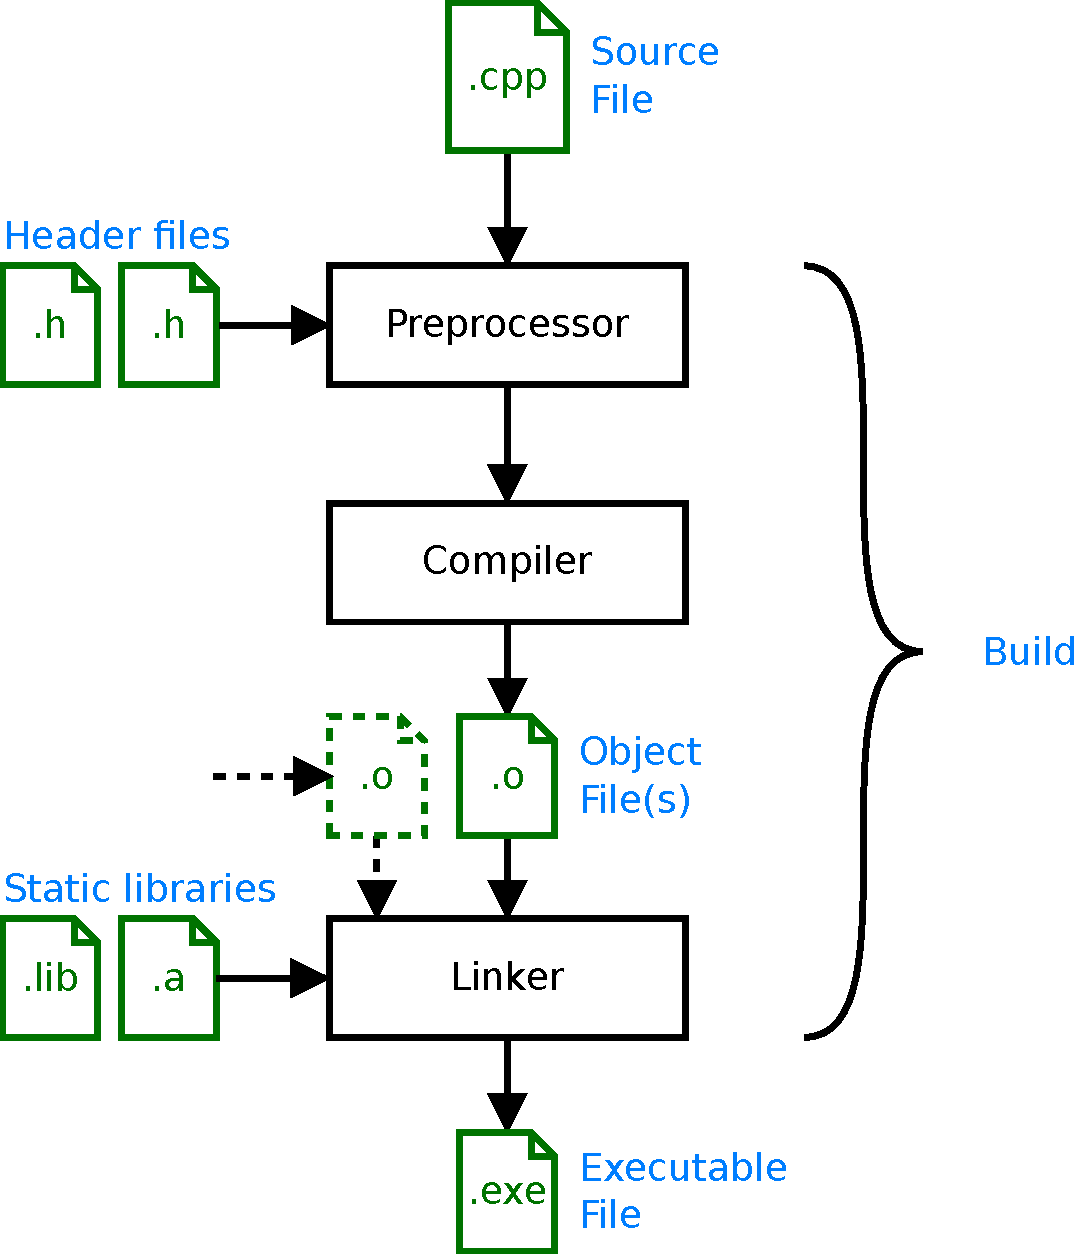
\includegraphics[scale=0.35]{figures/compilation_process_build}
%	\end{center}
%\end{frame}

%\begin{frame}
%\frametitle{Running process}
%\begin{center}
%	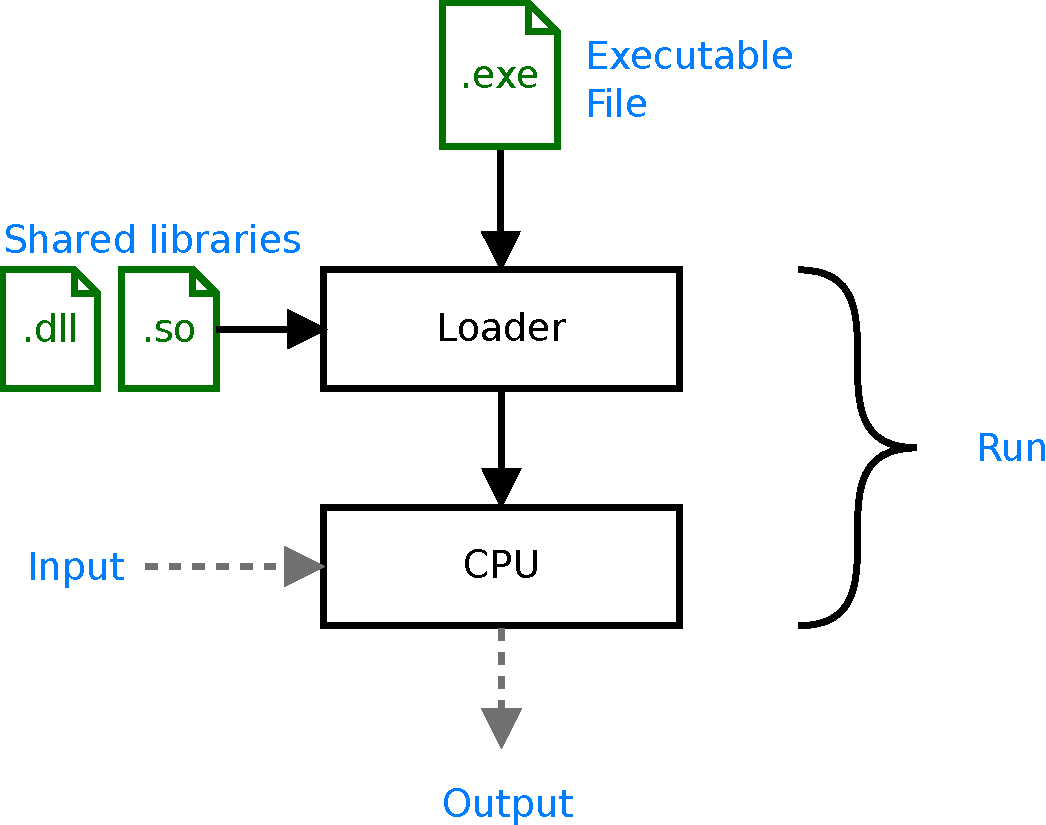
\includegraphics[scale=0.35]{figures/compilation_process_run}
%	\end{center}
%\end{frame}

\begin{frame}
\frametitle{Build \& run}
\begin{center}
	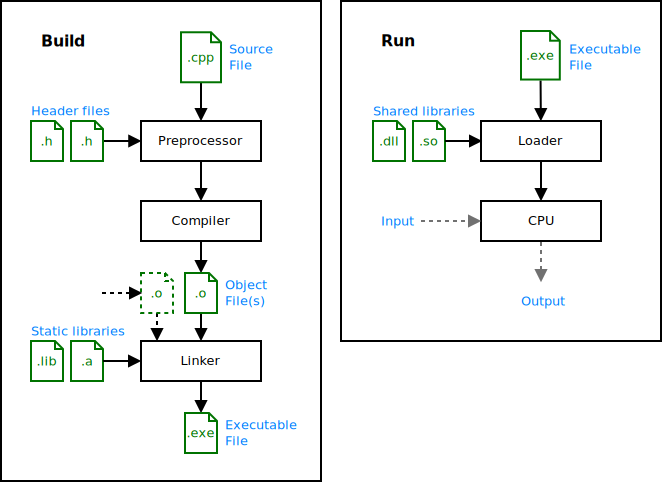
\includegraphics[scale=0.3]{figures/compilation_process3}
	\end{center}
\end{frame}

\begin{frame}
\frametitle{Compile, link and load}
\itemized{
	%\item The \emph{preprocessor} processes file inclusion and other \# directives.
	\item The \emph{compiler} translates source files (.cpp) into object files (.o).
	\item The \emph{linker} gathers information to link object files (.o) together with static libraries, producing an executable file (.exe).
	\item The \emph{loader} connects the executable file (.exe) with shared libraries (.so).
}
\end{frame}
%
%%%%%%%%%%%%%%%%%%%%%%%%%%%%%%%%%%%%%%%%%%%%%%%%%%%%%%%%%%%%%%%%%%%%%%%%%%%%%
%%%%% Hello world %%%%%%%%%%%%%%%%%%%%%%%%%%%%%%%%%%%%%%%%%%%%%%%%%%%%%%%%%%%
%%%%%%%%%%%%%%%%%%%%%%%%%%%%%%%%%%%%%%%%%%%%%%%%%%%%%%%%%%%%%%%%%%%%%%%%%%%%%
\begin{frame}
\pointedsl{Hello World!}
\end{frame}

\begin{frame}[fragile]
\frametitle{Hello World}
\begin{lstlisting}
#include<iostream>
// A comment
int main(int argc, char **argv){
    std::cout << "Hello world!\n";
    return 0;
}
\end{lstlisting}
\misc{
	Outputs "Hello world!" to the console and exits.
}
\end{frame}

%%%%%%%%%%%%%%%%%%%%%%%%%%%%%%%%%%%%%%%%%%%%%%%%%%%%%%%%%%%%%%%%%%%%%%%%%%%%%
%%%%% Pre-processor %%%%%%%%%%%%%%%%%%%%%%%%%%%%%%%%%%%%%%%%%%%%%%%%%%%%%%%%%
%%%%%%%%%%%%%%%%%%%%%%%%%%%%%%%%%%%%%%%%%%%%%%%%%%%%%%%%%%%%%%%%%%%%%%%%%%%%%
\begin{frame}[fragile]
\frametitle{Pre-processor instructions}
\begin{lstlisting}
#include<iostream>
\end{lstlisting}
\misc{
	Lines starting with a `\#' (pound) are instructions parsed by the \emph{pre-processor} such as
	\begin{itemize}
	\item \textbf{\#include} specifies a file to be included at this line.
	\item \textbf{\#if, \#ifdef, \#endif} conditionally uses a block of code.
	\item \textbf{\#define} creates an alias for an expression.
	\end{itemize}
}
\end{frame}

%%%%%%%%%%%%%%%%%%%%%%%%%%%%%%%%%%%%%%%%%%%%%%%%%%%%%%%%%%%%%%%%%%%%%%%%%%%%%
%%%%% Comments %%%%%%%%%%%%%%%%%%%%%%%%%%%%%%%%%%%%%%%%%%%%%%%%%%%%%%%%%%%%%%
%%%%%%%%%%%%%%%%%%%%%%%%%%%%%%%%%%%%%%%%%%%%%%%%%%%%%%%%%%%%%%%%%%%%%%%%%%%%%
\begin{frame}[fragile]
\frametitle{Comments}
\begin{lstlisting}[firstnumber=2]
// A comment (up to the end of the line)
\end{lstlisting}
\stext{or}
\begin{lstlisting}[firstnumber=2]
/* A comment 
possibly spanning
multiple lines */
\end{lstlisting}
\misc{
	are two types of comments, which the compiler ignores.
}
\end{frame}

%%%%%%%%%%%%%%%%%%%%%%%%%%%%%%%%%%%%%%%%%%%%%%%%%%%%%%%%%%%%%%%%%%%%%%%%%%%%%
%%%%% Main function %%%%%%%%%%%%%%%%%%%%%%%%%%%%%%%%%%%%%%%%%%%%%%%%%%%%%%%%%
%%%%%%%%%%%%%%%%%%%%%%%%%%%%%%%%%%%%%%%%%%%%%%%%%%%%%%%%%%%%%%%%%%%%%%%%%%%%%
\begin{frame}[fragile]
\frametitle{Main function}
\begin{lstlisting}[firstnumber=3]
int main(int argc, char **argv){
    ...
    return 0;
}
\end{lstlisting}
\misc{
	defines a function named \ctext{main} which
	\begin{itemize}
		\item takes two arguments \ctext{argc} and \ctext{argv},
		\item returns an integer value (\ctext{int} in front).
	\end{itemize}
	\phantom{.}
}
\end{frame}

\begin{frame}[fragile]
\frametitle{Main function (2)}
\begin{lstlisting}[firstnumber=3]
int main(int argc, char **argv){
    ...
    return 0;
}
\end{lstlisting}
\misc{
	The \ctext{main} function is called when the program starts, with
	\begin{itemize}
		\item \ctext{argc}, the number of arguments
		\item \ctext{argv}, the arguments (array of strings)
	\end{itemize}
	and returns an integer code ($0=$ success).
}
\end{frame}

%%%%%%%%%%%%%%%%%%%%%%%%%%%%%%%%%%%%%%%%%%%%%%%%%%%%%%%%%%%%%%%%%%%%%%%%%%%%%
%%%%% Output statement %%%%%%%%%%%%%%%%%%%%%%%%%%%%%%%%%%%%%%%%%%%%%%%%%%%%%%
%%%%%%%%%%%%%%%%%%%%%%%%%%%%%%%%%%%%%%%%%%%%%%%%%%%%%%%%%%%%%%%%%%%%%%%%%%%%%
\begin{frame}[fragile]
\frametitle{Output statement}
\begin{lstlisting}[firstnumber=4]
std::cout << "Hello world!\n";
\end{lstlisting}
\misc{
\begin{itemize}
	\item \ctext{std} is the standard \emph{namespace}.
	\item \ctext{cout} is a \emph{Stream} object.
	\item \ctext{<<} is the output operator of \emph{Stream}.
	\item \ctext{"Hello world"} is the string being output.
\end{itemize}
}
\end{frame}
%
%%%%%%%%%%%%%%%%%%%%%%%%%%%%%%%%%%%%%%%%%%%%%%%%%%%%%%%%%%%%%%%%%%%%%%%%%%%%%
%%%%% Basic C++ %%%%%%%%%%%%%%%%%%%%%%%%%%%%%%%%%%%%%%%%%%%%%%%%%%%%%%%%%%%%%
%%%%%%%%%%%%%%%%%%%%%%%%%%%%%%%%%%%%%%%%%%%%%%%%%%%%%%%%%%%%%%%%%%%%%%%%%%%%%
\begin{frame}
\pointedsl{
	Basics
}
\end{frame}

% TODO
% Content:
% 1. Variables (declaration, assignment, operations)
% 2. Types (list: char, short, int, float, double, bool, void; typedef)
% 3. Expressions (unary, binary, arithmetic, comparator, bitwise)
% 4. Conditions (if, else if, else)
% 5. Loops (for, while, do while)
% 6. Arrays
% 7. Functions (declaration, definition, signature /!\ types -> diff fun)

%%%%%%%%%%%%%%%%%%%%%%%%%%%%%%%%%%%%%%%%%%%%%%%%%%%%%%%%%%%%%%%%%%%%%%%%%%%%%
\lstset{numbers=none}
\begin{frame}[fragile]
\frametitle{Variables}
\begin{lstlisting}
int x; // declare a variable of type "int"
x = 7; // assign a value to "x"
int y = 2; // declare and assign 2 to "y"
y = y * 2; // multiply by 2, then reassign
y *= 2; // shorter version of above
int z = (y - 2) * x; // z equals 42
\end{lstlisting}
\misc{
	\textbf{Variables} are used to store data.
	
	Each variable posesses 
	\begin{itemize}
		\item a \emph{name} (\ctext{x}, \ctext{y}, \ctext{z})
		\item a \emph{type} (\ctext{int} for integer)
	\end{itemize}
	that enable the program to locate and interpret the data.
}
\end{frame}

%%%%%%%%%%%%%%%%%%%%%%%%%%%%%%%%%%%%%%%%%%%%%%%%%%%%%%%%%%%%%%%%%%%%%%%%%%%%%
\begin{frame}[fragile]
\frametitle{Variable types}
\begin{center}
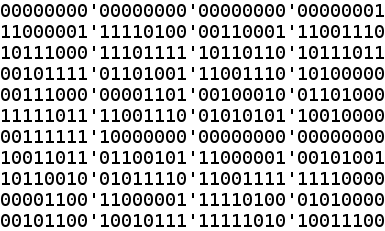
\includegraphics[width=0.6\textwidth]{figures/bits_black}
\end{center}
\misc{
	Computer data consists of sequences of '0' and '1' (bits).
	
	The type of a variable provides an interpretation of the data sequence. Without a type, the bits may mean anything.
}
\end{frame}

\begin{frame}[fragile]
\frametitle{Variable types}
\misc{
	Fundamental types include:
	\begin{itemize}
		\item \textbf{Integer types}: \ctext{char}${}^{(*)}$, \ctext{short}, \ctext{int}, \ctext{long} \\(each in \ctext{signed} or \ctext{unsigned} version)
		\item \textbf{Floating point types}: \ctext{float}, \ctext{double}
		\item \textbf{Boolean type:} \ctext{bool}
	\end{itemize}
	Each has a specific \emph{size} in memory and can only represent a limited amount of distinct values (the type \emph{range}).
}
\begin{lstlisting}
unsigned int n = 1; bool f = true;
char c = 'a'; double pi = 3.14159;
\end{lstlisting}
\end{frame}

\begin{frame}[fragile]
\frametitle{Variable types}
\begin{center}
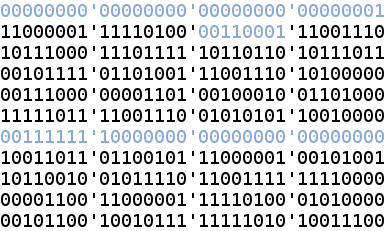
\includegraphics[width=0.6\textwidth]{figures/bits}
\end{center}
\lstset{
	xleftmargin=3cm
}
\begin{lstlisting}
int i = 1;
char c = '1';
float f = 1.0f;
\end{lstlisting}
\end{frame}

%%%%%%%%%%%%%%%%%%%%%%%%%%%%%%%%%%%%%%%%%%%%%%%%%%%%%%%%%%%%%%%%%%%%%%%%%%%%%
\begin{frame}[fragile]
\frametitle{Operators}
\misc{
	Each type has a set of (unary and binary) \textbf{operators}.
}
\begin{columns}[c]
  \begin{column}{0.5\textwidth}
\begin{lstlisting}
// arithmetic
// for numbers
+ - * / %
// bitwise
// for integers
& | ^ ~ >> <<
// incr- decrement
// for integers
++ --
\end{lstlisting}
  \end{column}
  \begin{column}{0.5\textwidth}
\begin{lstlisting}
// comparison
// producing bool
== != < <= > >=
// logical
// for bool
! || &&
// accessors
. :: * & ->
, [] ()
\end{lstlisting}
  \end{column}
\end{columns}
\end{frame}

\begin{frame}[fragile]
\frametitle{Operators}
\misc{
	When creating new types, one can overload the operator's behavior.
}
\begin{lstlisting}
std::cout << "Hello world!\n";
int input_number;
std::cin >> input_number;
\end{lstlisting}
\misc{
	For example, \ctext{Stream} objects use \ctext{<<} and \ctext{>>} as
	output and input operators.
}
\end{frame}

%%%%%%%%%%%%%%%%%%%%%%%%%%%%%%%%%%%%%%%%%%%%%%%%%%%%%%%%%%%%%%%%%%%%%%%%%%%%%
\begin{frame}[fragile]
\frametitle{Sequential flow}
\misc{
	The simplest programs are \textbf{sequential}: they execute a sequence of statements in the order they are written.
}
\end{frame}

\begin{frame}[fragile]
\frametitle{Sequential flow}
\begin{columns}[c]
  \begin{column}{0.5\textwidth}
  \hfill
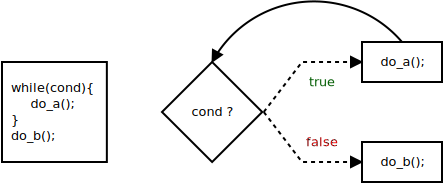
\includegraphics[scale=0.5]{figures/flow}
  \end{column}
  \begin{column}{0.5\textwidth}
\begin{lstlisting}
statement_1;
statement_2;
...
statement_N;

// Question:
// How to act
// according to
// the input?
\end{lstlisting}
  \end{column}
\end{columns}
\end{frame}

\begin{frame}[fragile]
\frametitle{Sequential flow}
\misc{
	The two main ways of breaking this sequential behavior are
	\begin{enumerate}
		\item \textbf{conditions} that execute statements only if a condition is met (or not) and
		\item \textbf{loops} that repeatedly execute statements until a specific state is reached (modeled as a condition).
	\end{enumerate}
}
\end{frame}

%%%%%%%%%%%%%%%%%%%%%%%%%%%%%%%%%%%%%%%%%%%%%%%%%%%%%%%%%%%%%%%%%%%%%%%%%%%%%
\begin{frame}[fragile]
\frametitle{Conditional flow}
\begin{columns}[c]
  \begin{column}{0.5\textwidth}
  \hfill
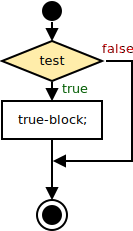
\includegraphics[scale=0.5]{figures/flow-ifthen}
  \end{column}
  \begin{column}{0.5\textwidth}
\begin{lstlisting}
if( test ){
  true_block;
}

// Question:
// Special action
// when the test
// fails?
\end{lstlisting}
  \end{column}
\end{columns}
\end{frame}

\begin{frame}[fragile]
\frametitle{Conditional flow}
\begin{columns}[c]
  \begin{column}{0.5\textwidth}
  \hfill
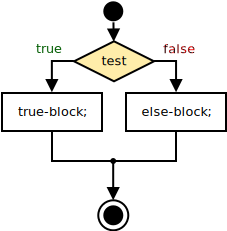
\includegraphics[scale=0.5]{figures/flow-ifelse}
  \end{column}
  \begin{column}{0.5\textwidth}
\begin{lstlisting}
if( test ){
  true_block;
} else {
  else_block;
}

// Note:
// Can be chained
// using
// else if(test)
\end{lstlisting}
  \end{column}
\end{columns}
\end{frame}

%%%%%%%%%%%%%%%%%%%%%%%%%%%%%%%%%%%%%%%%%%%%%%%%%%%%%%%%%%%%%%%%%%%%%%%%%%%%%
\begin{frame}[fragile]
\frametitle{Iterative flow: do-while}
\begin{columns}[c]
  \begin{column}{0.5\textwidth}
  \hfill
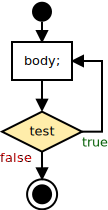
\includegraphics[scale=0.5]{figures/flow-do}
  \end{column}
  \begin{column}{0.5\textwidth}
\begin{lstlisting}
do {
  body;
} while( test );

// Question:
// How to check
// the test
// before body?
\end{lstlisting}
  \end{column}
\end{columns}
\end{frame}

\begin{frame}[fragile]
\frametitle{Iterative flow: while-loop}
\begin{columns}[c]
  \begin{column}{0.5\textwidth}
  \hfill
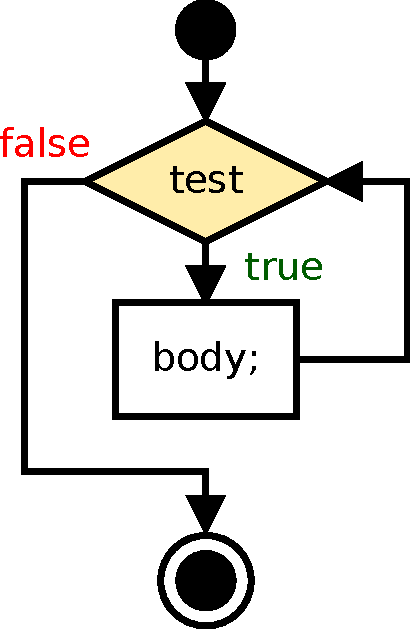
\includegraphics[scale=0.5]{figures/flow-while}
  \end{column}
  \begin{column}{0.5\textwidth}
\begin{lstlisting}
while(test){
  body;
}

// e.g.
while(i > 0){
  ...
  --i;
}
\end{lstlisting}
  \end{column}
\end{columns}
\end{frame}

\begin{frame}[fragile]
\frametitle{Iterative flow: for-loop}
\begin{columns}[c]
  \begin{column}{0.5\textwidth}
  \hfill
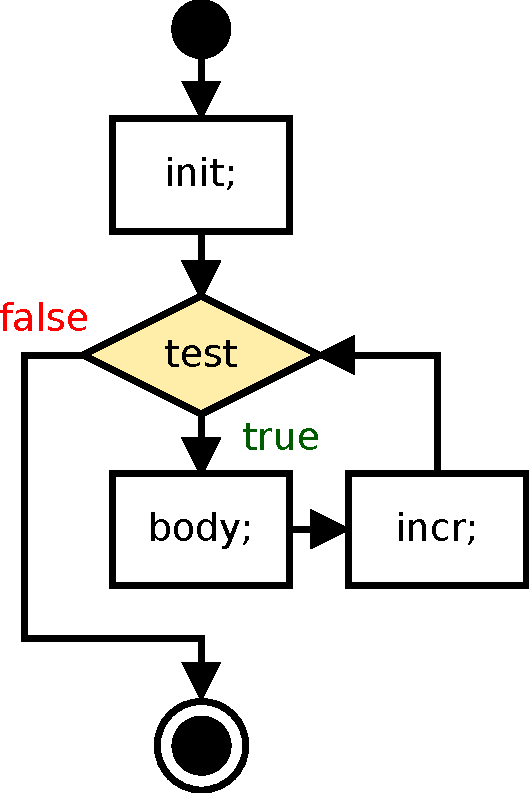
\includegraphics[scale=0.5]{figures/flow-for}
  \end{column}
  \begin{column}{0.5\textwidth}
\begin{lstlisting}
// for (a; b; c){}
for(init;
    test;
    incr){
  body;
}

// e.g.
for(int i = 0;
    i < 5; ++i){
  // loops 5 times
}
\end{lstlisting}
  \end{column}
\end{columns}
\end{frame}

%%%%%%%%%%%%%%%%%%%%%%%%%%%%%%%%%%%%%%%%%%%%%%%%%%%%%%%%%%%%%%%%%%%%%%%%%%%%%
\begin{frame}[fragile]
\frametitle{Loops, variables \& indexing}
\misc{
	Loops are important when processing a lot of similar data.
}
\begin{lstlisting}
int N = 0;
for(int i = 1; i < 100; ++i){
  N += i; // sum from 1 to 100
}
\end{lstlisting}
\misc{
	Here \ctext{N} refers to the same location
	whatever the value of \ctext{i}. What if we
	want a variable that depends on \ctext{i}?
}
\end{frame}

\begin{frame}[fragile]
\frametitle{Arrays}
\begin{columns}[c]
  \begin{column}{0.5\textwidth}
\lstset{numbers=left}
\begin{lstlisting}
int a[3] = { 1, 0 };
a[1] = 42;
// a[2] == 0
\end{lstlisting}
  \end{column}
  \begin{column}{0.5\textwidth}
    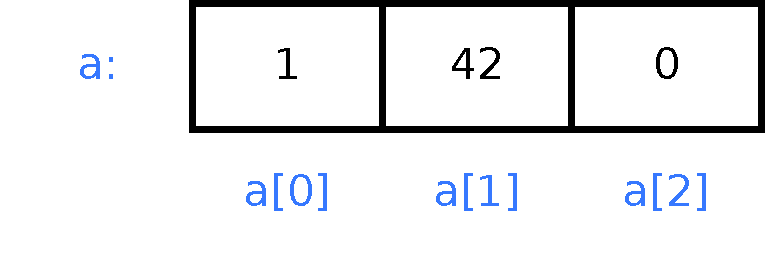
\includegraphics[width=0.95\textwidth]{figures/array0}
  \end{column}
\end{columns}
\misc{
	\emph{Arrays} are continuous blocks of memory that store multiple elements of a same type. They use $0$-based indexing.
	
	They are the storage of choice for multiple instances of a data type.
}
\end{frame}

%%%%%%%%%%%%%%%%%%%%%%%%%%%%%%%%%%%%%%%%%%%%%%%%%%%%%%%%%%%%%%%%%%%%%%%%%%%%%
\begin{frame}[fragile]
\frametitle{Functions}
\misc{
	Functions are pieces of program that can be executed as a whole.
}
\begin{lstlisting}
// How to get sum of integers
// from A to B?
int sum = 0;
for(int i = A; i <= B; ++i)
  sum += i;
  
// and from C to D?
// Copy code again?
\end{lstlisting}
\end{frame}

\begin{frame}[fragile]
\frametitle{Functions}
\begin{lstlisting}
int intSum(int A, int B){
  int sum = 0;
  for(int i = A; i <= B; ++i)
    sum += i;
  return sum;
}
\end{lstlisting}
\misc{
	Here \ctext{intSum} is a function that:
	\begin{itemize}
		\item takes two integer arguments \ctext{A} and \ctext{B}
		\item return the sum of integers between \ctext{A} and \ctext{B}
	\end{itemize}
}
\end{frame}

\begin{frame}[fragile]
\frametitle{Functions}
\begin{lstlisting}
// declare function
// (define it somewhere else)
int intSum(int, int);

// use function
int x = intSum(0, 100);
int y = x + intSum(101, 200);
// y == intSum(0, 200)
\end{lstlisting}
\misc{
	Functions must be \textbf{declared} before being used
	just like variables.
}
\end{frame}

\begin{frame}[fragile]
\frametitle{Functions}
\begin{lstlisting}
// /!\ different functions
int intSum(int, int);
int intSum(float);

// redeclare
int intSum(int x, int y);
// Note: argument names
// are irrelevant
\end{lstlisting}
\misc{
	They can be declared multiple times
	as long as the signature (name + types)
	match.
}
\end{frame}

%%%%%%%%%%%%%%%%%%%%%%%%%%%%%%%%%%%%%%%%%%%%%%%%%%%%%%%%%%%%%%%%%%%%%%%%%%%%%
%%%%% Pointers %%%%%%%%%%%%%%%%%%%%%%%%%%%%%%%%%%%%%%%%%%%%%%%%%%%%%%%%%%%%%%
%%%%%%%%%%%%%%%%%%%%%%%%%%%%%%%%%%%%%%%%%%%%%%%%%%%%%%%%%%%%%%%%%%%%%%%%%%%%%
\begin{frame}
\pointedsl{
	Pointers
}
\end{frame}

%%%%%%%%%%%%%%%%%%%%%%%%%%%%%%%%%%%%%%%%%%%%%%%%%%%%%%%%%%%%%%%%%%%%%%%%%%%%%
\begin{frame}[fragile]
\frametitle{Passing by value}
\begin{lstlisting}
void swap_wrong(int x, int y){
    int tmp = x;
    x = y;
    y = tmp;
}
int a = 1, b = 2;
swap_wrong(a, b);
// did not work! a=1, b=2
\end{lstlisting}
\misc{
	Function arguments are \textbf{passed by value} (copy of value). We need pointers to modify \ctext{a} and \ctext{b} in the code above.
}
\end{frame}

\begin{frame}[fragile]
\frametitle{Using pointers}
\begin{lstlisting}
void swap_ptr(int *x, int *y){
    int tmp = *x;
    *x = *y;
    *y = tmp;
}
int a = 1, b = 2;
swap_ptr(&a, &b);
// now a=2, b=1
\end{lstlisting}
\misc{
	\ctext{\&a} uses the \textbf{reference} operator to get the adresse of \ctext{a}.
	
	\ctext{*x} uses the \textbf{dereference} operator to get / set the value at the adress given by \ctext{x}.
}
\end{frame}

\begin{frame}[fragile]
\frametitle{References}
\begin{lstlisting}
// passed by reference
void swap_ref(int &x, int &y){
    int tmp = x;
    x = y;
    y = tmp;
}
int a = 1, b = 2;
swap_ref(a, b);
// good! a=2, b=1
\end{lstlisting}
\misc{
	\emph{References} are syntactic sugar for pointers when passing variables to functions or retrieving the value they return.
}
\end{frame}


%%%%%%%%%%%%%%%%%%%%%%%%%%%%%%%%%%%%%%%%%%%%%%%%%%%%%%%%%%%%%%%%%%%%%%%%%%%%%
\begin{frame}[fragile]
\frametitle{Pointer arithmetic}
\begin{columns}[c]
  \begin{column}{0.5\textwidth}
\lstset{language=C++,numbers=left}
\begin{lstlisting}
int a[5] = { 1 };
int *b = &a[0];
int *c = b + 3;
*c = 42; // or c[0]
c[1] = 5;
\end{lstlisting}
  \end{column}
  \begin{column}{0.5\textwidth}
    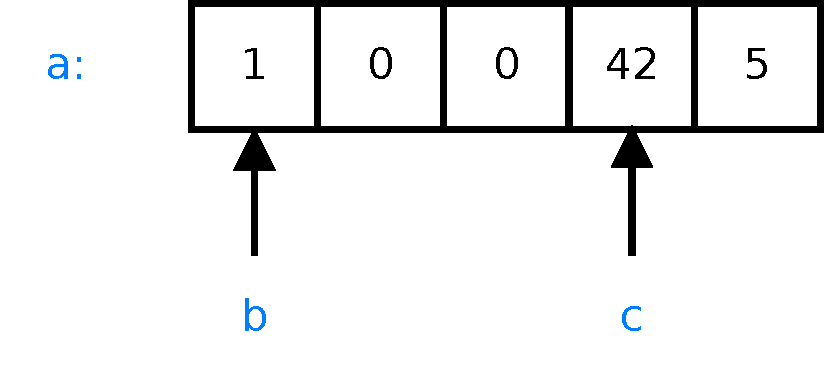
\includegraphics[width=\textwidth]{figures/array.pdf}
  \end{column}
\end{columns}
\misc{
	\begin{itemize}
		\item Accessing a pointer as an array
		\item Pointer arithmetic according to array indexing
	\end{itemize}
	
	\textbf{Warning!} A pointer value is the byte address and types have different sizes which can be found using \ctext{sizeof(mytype)}.
}
\end{frame}

%
%%%%%%%%%%%%%%%%%%%%%%%%%%%%%%%%%%%%%%%%%%%%%%%%%%%%%%%%%%%%%%%%%%%%%%%%%%%%%
%%%%% Templating %%%%%%%%%%%%%%%%%%%%%%%%%%%%%%%%%%%%%%%%%%%%%%%%%%%%%%%%%%%%
%%%%%%%%%%%%%%%%%%%%%%%%%%%%%%%%%%%%%%%%%%%%%%%%%%%%%%%%%%%%%%%%%%%%%%%%%%%%%
\begin{frame}
\pointedsl{
	Templating
}
\end{frame}

%
% Content:
% 1. Generic type
% 2. Template type inferrence
% 3. Template specialization

%%%%%%%%%%%%%%%%%%%%%%%%%%%%%%%%%%%%%%%%%%%%%%%%%%%%%%%%%%%%%%%%%%%%%%%%%%%%%
\begin{frame}[fragile]
\frametitle{Templating}
\begin{lstlisting}
template<typename T>
T sum(T a, T b){
    T c = a + b;
    return c;
}
\end{lstlisting}
\misc{
	Function (and class) \emph{templates} provides a way to abstract the notion of type.
	
	Here, the type \ctext{T} is resolved by the compiler when \ctext{sum} is used.
  It only requires an operator \ctext{+} to work${}^*$.
}
\end{frame}

\begin{frame}[fragile]
\frametitle{Templating (2)}
\begin{lstlisting}
int c = sum(1, 2);
float d = sum(1.0f, 2.0f);
float e = sum<float>(1, 2.0f);
\end{lstlisting}
\misc{
	The type \ctext{T} can sometimes by inferred. When it cannot, one must specify it.
}
\end{frame}

\begin{frame}[fragile]
\frametitle{Templating (3)}
\begin{lstlisting}
template<>
bool sum<bool>(bool a, bool b){
    return a || b; // a or b
}
bool a = true, b = false;
bool c = sum(a, b);
// c == true
\end{lstlisting}
\misc{
	Templates can be specialized for a given type.
}
\end{frame}
%
%%%%%%%%%%%%%%%%%%%%%%%%%%%%%%%%%%%%%%%%%%%%%%%%%%%%%%%%%%%%%%%%%%%%%%%%%%%%%
%%%%% Templating %%%%%%%%%%%%%%%%%%%%%%%%%%%%%%%%%%%%%%%%%%%%%%%%%%%%%%%%%%%%
%%%%%%%%%%%%%%%%%%%%%%%%%%%%%%%%%%%%%%%%%%%%%%%%%%%%%%%%%%%%%%%%%%%%%%%%%%%%%
\begin{frame}
\pointedsl{
	Classes
}
\end{frame}

%
% Content:
% 1. Basic class usage
% 2. Class variables & method declaration
% 3. Class definition
% 4. Constructor (default, copy, other), destructor
% 5. Accessors (public, protected, private)
% 6. Instance and static members
% 7. Operators and overloading

%%%%%%%%%%%%%%%%%%%%%%%%%%%%%%%%%%%%%%%%%%%%%%%%%%%%%%%%%%%%%%%%%%%%%%%%%%%%%
\begin{frame}[fragile]
\frametitle{Basic class usage}
\begin{lstlisting}
struct point {
  int x, y;
}; // don't forget ;

point p1, p2;
p1.x = 1;
p1.y = 2;
p2 = p1; // copy
p2.y = 2;
\end{lstlisting}
\misc{
	Classes (keyword \ctext{class}) and structures (keyword \ctext{struct}) describe custom types made of properties (here \ctext{x} and \ctext{y}).
}
\end{frame}

%%%%%%%%%%%%%%%%%%%%%%%%%%%%%%%%%%%%%%%%%%%%%%%%%%%%%%%%%%%%%%%%%%%%%%%%%%%%%
\begin{frame}[fragile]
\frametitle{Class member declaration}
\begin{lstlisting}
// declaration
struct vec {
    float val[2]; // variable
    // instance method:
    float sqLength() const;
    // static method:
    static vec constant(float a);
};
\end{lstlisting}
\misc{
	They can have specific methods (\ctext{sqLength}, \ctext{constant}).
}
\end{frame}

%%%%%%%%%%%%%%%%%%%%%%%%%%%%%%%%%%%%%%%%%%%%%%%%%%%%%%%%%%%%%%%%%%%%%%%%%%%%%
\begin{frame}[fragile]
\frametitle{Class definition}
\begin{lstlisting}
// definition
float vec::sqLength() {
    float sum = 0;
    for(int i = 0; i < dim; ++i)
        sum += val[i] * val[i];
    return sum;
}
\end{lstlisting}
\misc{
	The methods can be defined outside of the declaration.
	
	The usual pattern is:
	\begin{itemize}
		\item declare class in \ctext{classname.h}
		\item define class in \ctext{classname.cpp}
	\end{itemize}
}
\end{frame}

%%%%%%%%%%%%%%%%%%%%%%%%%%%%%%%%%%%%%%%%%%%%%%%%%%%%%%%%%%%%%%%%%%%%%%%%%%%%%
\begin{frame}[fragile]
\frametitle{Constructors and destructor}
\misc{
	Some methods are special, including
	\begin{itemize}
		\item the \textbf{default constructor} which is called for instances without specific initialization
		\item the \textbf{copy constructor} which is used for passing argument by value and when assigning a copy of a variable to a new variable
		\item the \textbf{destructor} which is called when the instance is deleted
	\end{itemize}
}
\end{frame}

%%%%%%%%%%%%%%%%%%%%%%%%%%%%%%%%%%%%%%%%%%%%%%%%%%%%%%%%%%%%%%%%%%%%%%%%%%%%%
\begin{frame}[fragile]
\frametitle{Instance creation}
\begin{lstlisting}
struct point {
  int x, y;

  point(int a, int b); // my constructor
  point(); // default constructor
  point(const point &p); // copy constructor
  ~point(); // destructor
};

point a(1, 2); // my constructor
point b; // default constructor
point c(a); // copy constructor
// assignment using copy constructor
point d = e;
\end{lstlisting}
\end{frame}

%%%%%%%%%%%%%%%%%%%%%%%%%%%%%%%%%%%%%%%%%%%%%%%%%%%%%%%%%%%%%%%%%%%%%%%%%%%%%
\begin{frame}[fragile]
\frametitle{Accessors}
\misc{
	Members of classes can be 
	\begin{itemize}
		\item \ctext{public}: can be accessed from everywhere, 
		\item \ctext{protected}: can only be accessed by classes that extend it, or 
		\item \ctext{private}: can only be accessed by methods of that instance
	\end{itemize}
	
	By default, \ctext{struct}'s have every member \ctext{public} whereas \ctext{class}'es default to \ctext{private}.
}
\end{frame}

%%%%%%%%%%%%%%%%%%%%%%%%%%%%%%%%%%%%%%%%%%%%%%%%%%%%%%%%%%%%%%%%%%%%%%%%%%%%%
\begin{frame}[fragile]
\frametitle{Accessors}
\lstset{
  xrightmargin=0cm
}
\begin{columns}[c]
  \begin{column}{0.5\textwidth}
\begin{lstlisting}
struct point {
  int x, y;
  void print();
private:
  void debug();
};

// ok:
point a;
a.print();
// error:
a.debug();
\end{lstlisting}
  \end{column}
  \begin{column}{0.5\textwidth}
\lstset{ numbers=none, xleftmargin=0cm }
\begin{lstlisting}
class vec {
  int val[2];
public:
  vec(int a, int b);
  int sqLength();
};

// ok:
vec b(1, 2);
int l = b.sqLength();
// error:
b.val[0] = 1;
\end{lstlisting}
  \end{column}
\end{columns}
\end{frame}

%%%%%%%%%%%%%%%%%%%%%%%%%%%%%%%%%%%%%%%%%%%%%%%%%%%%%%%%%%%%%%%%%%%%%%%%%%%%%
\begin{frame}[fragile]
\frametitle{Static members}
\misc{
	Normal variable and methods are relative to the instance of the class that stores them.
	
	The keyword \ctext{static} can be used to declare variables or methods that are relative to the namespace of the class, shared by all instances.
	
	Accessing and using static members is done using the namespace operator \ctext{::}.
}
\end{frame}

%%%%%%%%%%%%%%%%%%%%%%%%%%%%%%%%%%%%%%%%%%%%%%%%%%%%%%%%%%%%%%%%%%%%%%%%%%%%%
\begin{frame}[fragile]
\frametitle{Static members}
\begin{lstlisting}
struct id {
  const int value;
  id() : value(num++){}
  int count() { return num; }
private:
  static int num;
}
int id::num = 0;

id a, b;
// a.value == 0, b.value == 1
// a.count() == b.count() == 2
\end{lstlisting}
\end{frame}

%%%%%%%%%%%%%%%%%%%%%%%%%%%%%%%%%%%%%%%%%%%%%%%%%%%%%%%%%%%%%%%%%%%%%%%%%%%%%
\begin{frame}[fragile]
\frametitle{Operators}
\begin{lstlisting}
struct vec {
  int x, y;
  vec operator +(const vec &v) const {
    return vec(x + v.x, y + v.y);
  }
};

vec a, b;
...
vec c = a + b;
\end{lstlisting}
\misc{
	Operators can be overloaded to produce cleaner code.
	
	Beware of the excess!
}
\end{frame}
%
%%%%%%%%%%%%%%%%%%%%%%%%%%%%%%%%%%%%%%%%%%%%%%%%%%%%%%%%%%%%%%%%%%%%%%%%%%%%%
%%%%% C++ and Memory %%%%%%%%%%%%%%%%%%%%%%%%%%%%%%%%%%%%%%%%%%%%%%%%%%%%%%%%
%%%%%%%%%%%%%%%%%%%%%%%%%%%%%%%%%%%%%%%%%%%%%%%%%%%%%%%%%%%%%%%%%%%%%%%%%%%%%
\begin{frame}
\pointedsl{
	Stack / Heap
}
\end{frame}

% See http://stackoverflow.com/questions/79923/what-and-where-are-the-stack-and-heap
% See http://gribblelab.org/CBootcamp/7_Memory_Stack_vs_Heap.html
% See http://www.learncpp.com/cpp-tutorial/79-the-stack-and-the-heap/

%
% Content:
% 1. Stack -vs- heap
% 2. Stack: variable scope (when is the destructor called?)
% 3. Heap: new & delete (and memory leaks)
% 4. Heap: arrays with new and delete
% 5. Smart pointers

%%%%%%%%%%%%%%%%%%%%%%%%%%%%%%%%%%%%%%%%%%%%%%%%%%%%%%%%%%%%%%%%%%%%%%%%%%%%%
\begin{frame}[fragile]
\frametitle{Stack -vs- heap}
\misc{
	The \emph{stack} is a place where variables live and die depending on their location in the program.
	
	The \emph{heap} is the place where variables live (and die) independently of their location in the program.
}
\end{frame}

%%%%%%%%%%%%%%%%%%%%%%%%%%%%%%%%%%%%%%%%%%%%%%%%%%%%%%%%%%%%%%%%%%%%%%%%%%%%%

\begin{frame}[fragile]
\frametitle{Stack: life and death of a variable}
\begin{lstlisting}
int life_of_a_variable(bool b){ // b born
  int a = 0; // a born
  if(b){
    int c = 10; // c born
    ... // do other things
  } // c dead
  return a; // a copied, then dead
} // b dead
\end{lstlisting}
\misc{
	On the \emph{stack}, local variables die as soon as the program reaches back a level where the considered variables were not defined.
	
	They die with the call of their \emph{destructor}.
}
\end{frame}

%%%%%%%%%%%%%%%%%%%%%%%%%%%%%%%%%%%%%%%%%%%%%%%%%%%%%%%%%%%%%%%%%%%%%%%%%%%%%

\begin{frame}[fragile]
\frametitle{Using the stack}
\begin{center}
\B
\begin{tabular}{ll}
\B \textbf{Pro} & \B \textbf{Contra} \\\hline
\B Very fast access & \B \ctext{return} requires a copy \\
\B Managed life-cycle & \B Limited available memory \\
\B No memory fragmentation & \B Fixed-size arrays \\
\B & \B No re-allocation
\end{tabular}
\end{center}
\misc{
	The stack should be reserved for \textbf{simple} and \textbf{local} variables.
	
	\textbf{Heavy} or \textbf{size-varying} variables should be allocated on the heap.
}
\end{frame}

%%%%%%%%%%%%%%%%%%%%%%%%%%%%%%%%%%%%%%%%%%%%%%%%%%%%%%%%%%%%%%%%%%%%%%%%%%%%%
\begin{frame}[fragile]
\lstset{ numbers=none }
\frametitle{Heap: \ctext{new} and \ctext{delete}}
\begin{lstlisting}
// forward-declaration
class User; // with complex data

User *myself = new User("Alex");
// use myself, possibly return
//     from a function
// eventually delete:
delete myself;
\end{lstlisting}
\misc{
	Using \ctext{new} enforces that the variable is created on the heap.
	
	Instances created on the heap are not deleted automatically, the programmer must use \ctext{delete} on these instances to free the memory.
}
\end{frame}

\begin{frame}[fragile]
\lstset{ numbers=none }
\frametitle{Heap: \ctext{new} and \ctext{delete}}
\begin{lstlisting}
struct Image {
  int x, y;
  ...
  void resize(Size newSize);
};

Image *img = new Image;
img->x = 10; // same as (*img).x
img->y = 10; // same as (*img).y
img->resize(100, 100);
\end{lstlisting}
\misc{
	Instances on the heap are dealt with using pointers.
	
	Accessing their members is done using the \ctext{->} operator.
}
\end{frame}

%%%%%%%%%%%%%%%%%%%%%%%%%%%%%%%%%%%%%%%%%%%%%%%%%%%%%%%%%%%%%%%%%%%%%%%%%%%%%
\begin{frame}[fragile]
\frametitle{Heap: arrays with \ctext{new[]} and \ctext{delete[]}}
\begin{lstlisting}
// fibonacci sequence
int *fibSequence(int N){
  int *seq = new int[N];
  seq[0] = seq[1] = 1;
  for(int i = 2; i < N; ++i)
    seq[i] = seq[i-1] + seq[i-2];
  return seq;
}
\end{lstlisting}
\misc{
	Creating arrays on the heap (especially any array of variable size) is done using
	the \ctext{new[]} operator.
	
	Freeing uses the corresponding \ctext{delete[]} operator.
}
\end{frame}

%%%%%%%%%%%%%%%%%%%%%%%%%%%%%%%%%%%%%%%%%%%%%%%%%%%%%%%%%%%%%%%%%%%%%%%%%%%%%
\begin{frame}[fragile]
\frametitle{Smart pointers}
\begin{lstlisting}
#include<memory>
struct point {
  int x, y;
  point(int, int);
};

std::auto_ptr<point> ptr(new point(1, 2));
// no need to use delete!
\end{lstlisting}
\misc{
	Smart pointers are classes that wrap pointers and take care of the deallocation automatically.
}
\end{frame}

\begin{frame}[fragile]
\frametitle{Smart pointers}
\misc{
	Various flavors exist including
	\begin{itemize}
		\item \ctext{scoped\_ptr}: single instance that dies like a stack variable, and cannot be copied anywhere else
		\item \ctext{auto\_ptr}: single instance that dies like stack variables, but can be copied somewhere else
		\item \ctext{shared\_ptr}: pointer that is used at multiple locations, uses reference counting to die when there is no reference anymore
		\item \ctext{weak\_ptr}: instance similar to the shared version, but without reference count, and whose content may not exist anymore if the other instances all died
	\end{itemize}
}
\end{frame}

%
%%%%%%%%%%%%%%%%%%%%%%%%%%%%%%%%%%%%%%%%%%%%%%%%%%%%%%%%%%%%%%%%%%%%%%%%%%%%%
%%%%% Polymorphism %%%%%%%%%%%%%%%%%%%%%%%%%%%%%%%%%%%%%%%%%%%%%%%%%%%%%%%%%%
%%%%%%%%%%%%%%%%%%%%%%%%%%%%%%%%%%%%%%%%%%%%%%%%%%%%%%%%%%%%%%%%%%%%%%%%%%%%%
\begin{frame}
\pointedsl{
	Polymorphism
}
\end{frame}

% TODO
% Content:
% 1. Inheritance
% 2. Virtual methods
% 3. Pure virtual methods

%%%%%%%%%%%%%%%%%%%%%%%%%%%%%%%%%%%%%%%%%%%%%%%%%%%%%%%%%%%%%%%%%%%%%%%%%%%%%
\begin{frame}[fragile]
\frametitle{References}
\begin{lstlisting}
// passed by reference
void swap_ref(int &x, int &y){
    int tmp = x;
    x = y;
    y = tmp;
}
int a = 1, b = 2;
swap_ref(a, b);
// good! a=2, b=1
\end{lstlisting}
\misc{
	\emph{References} are syntactic sugar for pointers when passing variables to functions or retrieving the value they return.
}
\end{frame}
%
%%%%%%%%%%%%%%%%%%%%%%%%%%%%%%%%%%%%%%%%%%%%%%%%%%%%%%%%%%%%%%%%%%%%%%%%%%%%%
%%%%% Types and conversions %%%%%%%%%%%%%%%%%%%%%%%%%%%%%%%%%%%%%%%%%%%%%%%%%
%%%%%%%%%%%%%%%%%%%%%%%%%%%%%%%%%%%%%%%%%%%%%%%%%%%%%%%%%%%%%%%%%%%%%%%%%%%%%
\begin{frame}
\pointedsl{
	Conversions
}
\end{frame}

% TODO
% Content:
% 1. Conversion to base type
% 2. Conversion to super type: static_cast and dynamic_cast
% 3. reinterpret_cast, type(), (type)
% 4. const qualifier, const_cast
% 5. implicit and explicit conversions

%%%%%%%%%%%%%%%%%%%%%%%%%%%%%%%%%%%%%%%%%%%%%%%%%%%%%%%%%%%%%%%%%%%%%%%%%%%%%
\begin{frame}[fragile]
\frametitle{References}
\begin{lstlisting}
// passed by reference
void swap_ref(int &x, int &y){
    int tmp = x;
    x = y;
    y = tmp;
}
int a = 1, b = 2;
swap_ref(a, b);
// good! a=2, b=1
\end{lstlisting}
\misc{
	\emph{References} are syntactic sugar for pointers when passing variables to functions or retrieving the value they return.
}
\end{frame}
%
%%%%%%%%%%%%%%%%%%%%%%%%%%%%%%%%%%%%%%%%%%%%%%%%%%%%%%%%%%%%%%%%%%%%%%%%%%%%%
%%%%% Advanced C++ %%%%%%%%%%%%%%%%%%%%%%%%%%%%%%%%%%%%%%%%%%%%%%%%%%%%%%%%%%
%%%%%%%%%%%%%%%%%%%%%%%%%%%%%%%%%%%%%%%%%%%%%%%%%%%%%%%%%%%%%%%%%%%%%%%%%%%%%
\begin{frame}
\pointedsl{
	Advanced C++
}
\end{frame}

%%%%%%%%%%%%%%%%%%%%%%%%%%%%%%%%%%%%%%%%%%%%%%%%%%%%%%%%%%%%%%%%%%%%%%%%%%%%%
\begin{frame}[fragile]
\frametitle{References}
\begin{lstlisting}
// passed by reference
void swap_ref(int &x, int &y){
    int tmp = x;
    x = y;
    y = tmp;
}
int a = 1, b = 2;
swap_ref(a, b);
// good! a=2, b=1
\end{lstlisting}
\misc{
	\emph{References} are syntactic sugar for pointers when passing variables to functions or retrieving the value they return.
}
\end{frame}

%%%%%%%%%%%%%%%%%%%%%%%%%%%%%%%%%%%%%%%%%%%%%%%%%%%%%%%%%%%%%%%%%%%%%%%%%%%%%
\begin{frame}[fragile]
\frametitle{Templating}
\begin{lstlisting}
template< typename T >
T sum(T a, T b){
    T c = a + b;
    return c;
}
\end{lstlisting}
\misc{
	Function (and class) \emph{templates} provides a way to abstract the notion of type.
	
	Here, the type \ctext{T} is resolved by the compiler when \ctext{sum} is used.
	It only requires an operator \ctext{+} to work.
}
\end{frame}

%%%%%%%%%%%%%%%%%%%%%%%%%%%%%%%%%%%%%%%%%%%%%%%%%%%%%%%%%%%%%%%%%%%%%%%%%%%%%
\begin{frame}[fragile]
\frametitle{Templating (2)}
\begin{lstlisting}
int c = sum(1, 2);
float d = sum(1.0f, 2.0f);
float e = sum<float>(1, 2.0f);
\end{lstlisting}
\misc{
	The type \ctext{T} can sometimes by inferred. When it cannot, one must specify it.
}
\end{frame}

%%%%%%%%%%%%%%%%%%%%%%%%%%%%%%%%%%%%%%%%%%%%%%%%%%%%%%%%%%%%%%%%%%%%%%%%%%%%%
\begin{frame}[fragile]
\frametitle{Classes}
\begin{lstlisting}
// declaration
template <typename T, int dim>
struct vec {
    typedef vec<T, dim> this_type;
    T val[dim];
    vec(T a, T b);
    double sqLength() const;
    static this_type constant(T a);
};
\end{lstlisting}
\misc{
	Classes (keyword \ctext{class}) and structures (keyword \ctext{struct}) describe custom types made
	of properties (\ctext{val}) and methods (\ctext{sqLength}).
}
\end{frame}

\begin{frame}[fragile]
\frametitle{Classes (2)}
\begin{lstlisting}
// definitions
template <typename T, int dim>
double vec<T, dim>::sqLength() {
    T sum = 0;
    for(int i = 0; i < dim; ++i)
        sum += val[i] * val[i];
    return sum;
}
\end{lstlisting}
\misc{
	Definition of methods (including the constructor \ctext{vec} and/or its possible destructor \ctext{~vec} can be done separately.
}
\end{frame}

\begin{frame}[fragile]
\frametitle{Classes (3)}
\begin{lstlisting}
// type alias
typedef vec<float, 2> vec2f;

// class usage
vec2f a = vec2f::constant(2);
float d = a.sqLength(); // d=8
\end{lstlisting}
\misc{
	Static properties and methods are called with the namespace operator (\ctext{::}) whereas
	instance properties and methods are accessed with the dot operator.
}
\end{frame}

\begin{frame}[fragile]
\frametitle{Operator overloading}
\begin{lstlisting}
vec2f operator +(const vec2f &v1,
                 const vec2f &v2){
    vec2f x;
    for(int i = 0; i < 2; ++i)
        x.val[i] = v1.val[i] + v2.val[i];
    return x;
}

// usage
vec2f a, b;
// hidden: initialization of a and b
vec3f c = a + b;
\end{lstlisting}
\end{frame}


%%%%%%%%%%%%%%%%%%%%%%%%%
%%% ENDING %%%%%%%%%%%%%%
%%%%%%%%%%%%%%%%%%%%%%%%%

\fbckg{backgrounds/blank2}
\begin{frame}
  \thankyou   %%%% ending slide with thank you notice
\end{frame}

\newcommand{\resource}[2]{
  
\includegraphics[height=1em]{figures/C++-logo} \ \href{#1}{#2}
}
\begin{frame}
\sources{
\resource{http://ocw.mit.edu/courses/electrical-engineering-and-computer-science/6-096-introduction-to-c-january-iap-2011/index.htm}{Introduction to C++,  MIT OpenCourseWare}\\
\resource{http://www.cs.washington.edu/homes/tom/c++example/c++.pdf}{A Quick Introduction to C++, Thomas Anderson}\\
\resource{https://www3.ntu.edu.sg/home/ehchua/programming/index.html\#Cpp}{C/C++ Tutorials, Chua Hock-Chuan}\\
\resource{http://www.stroustrup.com/C++11FAQ.html}{C++11 Faq, Bjarne Stroustrup}
}
\end{frame}


\end{document}